\chapter{Eventos e Missões}

\section{Ocorrência Estranha no Discódromo}

\subsection{Contexto}
O Discódromo, uma das casas noturnas mais movimentadas de Barra das Garças, é conhecido por suas festas temáticas e sua atmosfera mística. O local atrai desde curiosos e turistas interessados em histórias sobrenaturais até seguidores de seitas locais e simpatizantes de teorias conspiratórias. Recentemente, a ANVESN recebeu denúncias anônimas de comportamentos estranhos observados durante essas festas, como convidados em transe e desaparecimentos repentinos.

\subsection{Missão}
A missão dos agentes é infiltrar-se na próxima festa temática, intitulada ``Noite do Véu'', que promete uma ``experiência de transcendência'' com músicas supostamente capazes de alterar o estado de consciência. Cláudia, a DJ residente, foi identificada como suspeita, pois rumores dizem que ela utiliza uma faixa musical específica para abrir um canal para outra dimensão. A ANVESN quer entender o que realmente acontece no Discódromo, neutralizar qualquer ameaça e impedir que entidades do Intraterra possam atravessar para a superfície.

\subsection{Informações e Pistas}
\begin{itemize}
    \item \textbf{Broche dos Intraterrenos}: Vários convidados estarão usando um broche discreto em formato de criatura subterrânea, indicando sua lealdade ao grupo de Bento, um conhecido líder conspirador. Os agentes podem interrogar esses convidados discretamente para entender o envolvimento de Bento e descobrir se eles sabem mais sobre o propósito da festa.

    \item \textbf{Convite para a Reunião Secreta}: Alguns dos frequentadores da festa terão convites para uma reunião privada que ocorrerá no final do evento, onde serão discutidas ``medidas de proteção para Barra das Garças''. Os agentes podem tentar obter um desses convites ou interrogar alguém que possua um, ganhando acesso à reunião onde informações cruciais sobre os intraterrenos poderão ser obtidas.

    \item \textbf{Música de Invocação}: Cláudia, a DJ, prepara uma faixa musical única para o encerramento da festa. Há relatos de que essa música contém frequências de som que alteram a percepção dos ouvintes e abrem brechas temporárias para o Intraterra. Os agentes devem observar os efeitos dessa música e, se necessário, interromper a performance para evitar a abertura completa do portal.
\end{itemize}

\subsection{Estrutura da Missão}
\begin{itemize}
    \item \textbf{Fase de Infiltração}: Os agentes entram no Discódromo como civis. Eles devem misturar-se à multidão, interagir com os convidados e reunir informações sobre os boatos da festa. Esse momento permite que eles estabeleçam contatos e identifiquem suspeitos.

    \item \textbf{Fase de Investigação}: Durante a festa, os agentes podem explorar os bastidores do Discódromo, incluindo a cabine da DJ e as áreas de staff. Nesses locais, é possível encontrar registros e notas que Cláudia usou para compor a música de invocação, talvez até com símbolos e idiomas incomuns. Eles também podem descobrir que Cláudia mantém contato com o grupo de Bento, sugerindo que ela é uma aliada do Intraterra.

    \item \textbf{Fase de Confronto}: Quando a faixa especial de invocação é tocada, alguns convidados entram em transe profundo e começam a agir de forma violenta ou incoerente. Entidades do Intraterra podem se manifestar de forma parcial, como sombras nas paredes ou formas nebulosas que ameaçam os presentes. Os agentes precisarão agir rápido para conter a situação, desligando o sistema de som e afastando os convidados afetados do local.
\end{itemize}

\subsection{Possíveis Complicações}
\begin{itemize}
    \item \textbf{Seguidores de Bento}: Alguns convidados podem ser membros leais do grupo de Bento e, ao perceberem a presença da ANVESN, tentarão atrapalhar as ações dos agentes, criando distrações ou confrontos.

    \item \textbf{Influência do Intraterra}: O ambiente do Discódromo pode começar a mostrar sinais de distorção dimensional, como sombras que se movem de maneira independente e mudanças temporárias na arquitetura do local. Isso aumenta a sensação de perigo e confunde os agentes.

    \item \textbf{Fuga de Cláudia}: Ao perceber que sua atuação está sendo interrompida, Cláudia pode tentar escapar pelos corredores dos bastidores, levando com ela documentos e registros de contatos com o Intraterra. Impedir sua fuga e recuperar esses materiais pode fornecer pistas importantes para futuras investigações.
\end{itemize}

\subsection{Conclusão da Missão}
Se os agentes conseguirem conter a situação, interrompendo a música de invocação e neutralizando as influências do Intraterra, a ANVESN ganhará controle sobre o Discódromo. Eles podem então investigar o local com calma, encontrando provas materiais da influência dos intraterrenos e informações sobre os próximos passos de Bento. Cláudia poderá ser presa e interrogada, fornecendo detalhes sobre a aliança com os Intraterrenos.

Por outro lado, se os agentes falharem em conter a situação, o Discódromo pode se tornar um ponto de atividade sobrenatural contínua, aumentando o acesso do Intraterra à superfície e exigindo uma intervenção de emergência da ANVESN para evitar uma catástrofe maior.


\section{Encontro com o ET}

Após coletar pistas, os agentes encontram o ET na floresta e descobrem que ele precisa da peça para consertar sua nave. O alienígena explica que não representa ameaça, mas está sendo perseguido pelos intraterrenos.

\subsection{Interação com o ET}

O ET pede aos agentes que recuperem a peça, guardada pelos intraterrenos na sala de monitoramento da caverna. Ele também pede proteção contra os intraterrenos, que temem sua presença.

\section{Confronto com os Intraterrenos}

Os agentes descobrem que Bento e os intraterrenos se organizam para capturar o ET. Eles devem decidir entre diplomacia ou confronto:

\begin{itemize}
    \item \textbf{Diplomacia}: Usar Empatia para explicar que o ET não representa risco.
    \item \textbf{Confronto}: Enfrentar os aliados de Bento e os intraterrenos, usando habilidades de combate.
\end{itemize}

\subsection{Encontros Sobrenaturais com Seres Fantásticos}

A presença de seres místicos e guardiões do folclore brasileiro nas redondezas de Barra das Garças pode se manifestar de várias formas, deixando pistas e rastros para os personagens interpretarem. Abaixo estão descritas cenas em que os personagens podem perceber a presença desses seres, criando uma atmosfera de mistério e aumentando a sensação de estar em um lugar onde o sobrenatural é parte do cotidiano.

\subsubsection{Curupira – Pegadas Reviradas e Sons da Floresta}

\textbf{Cena:} Ao atravessarem uma parte densa da floresta, os personagens notam pegadas reviradas, como se alguém tivesse caminhado de costas. Um silêncio repentino toma conta do local, seguido de uma risada leve e distante. À medida que avançam, sons de animais começam a ecoar ao redor, mas os personagens percebem que estão retornando ao ponto de partida, como se estivessem andando em círculos.

\textbf{Dicas de Presença:}  
\begin{itemize}
    \item Pegadas reviradas no chão, em áreas onde não há sinal de ninguém além dos personagens.
    \item Risadas leves, quase infantis, e sombras rápidas ao longe, como se alguém estivesse observando.
    \item Sons de animais que indicam que o Curupira está perto e prestes a intervir caso os personagens sigam em frente sem permissão.
\end{itemize}

\subsubsection{Saci-Pererê – Redemoinhos e Riso Travesso}

\textbf{Cena:} Durante uma caminhada ao entardecer, um pequeno redemoinho de folhas surge subitamente próximo aos personagens, girando ao redor deles antes de desaparecer. Logo em seguida, um dos personagens percebe que um item desapareceu de sua mochila. Uma gargalhada travessa ecoa entre as árvores e o redemoinho reaparece mais à frente, como se estivesse conduzindo o grupo a um ponto específico.

\textbf{Dicas de Presença:}  
\begin{itemize}
    \item Redemoinhos pequenos e estranhos que aparecem e desaparecem ao redor do grupo.
    \item Riso travesso e vozes sussurradas, como se o Saci estivesse pregando uma peça.
    \item Objetos desaparecendo ou trocados de lugar, obrigando os personagens a segui-lo para recuperar o que perderam.
\end{itemize}

\subsubsection{Boitatá – Um Fogo Brilhante que Dança na Escuridão}

\textbf{Cena:} Enquanto exploram um campo aberto próximo à floresta, os personagens avistam, ao longe, uma luz brilhante e alaranjada que se move em ziguezague. À medida que se aproximam, a luz intensifica-se, quase como se estivesse viva. Eles sentem um calor forte e veem que a luz toma a forma de uma serpente de fogo, observando-os de longe antes de desaparecer na escuridão.

\textbf{Dicas de Presença:}  
\begin{itemize}
    \item Luzes alaranjadas que se movem de maneira incomum, como se estivessem “patrulhando” a área.
    \item Calor intenso mesmo à distância, acompanhado de uma sensação de estar sendo observado.
    \item Marcas de queimaduras no solo, em forma de serpente, indicando o trajeto que o Boitatá percorreu.
\end{itemize}

\subsubsection{Mapinguari – O Forte Aroma e o Som da Vegetação Rasteira}

\textbf{Cena:} Na mata fechada, o grupo sente um cheiro insuportavelmente forte e desagradável, seguido por um barulho intenso de passos pesados na vegetação rasteira. De repente, um grito estridente ecoa pela floresta, e os personagens percebem a silhueta imensa de uma criatura ao longe. A vegetação densa balança, revelando apenas brevemente o contorno do Mapinguari, antes que ele desapareça na escuridão da floresta.

\textbf{Dicas de Presença:}  
\begin{itemize}
    \item Cheiro pungente que permeia o ambiente, acompanhado por barulhos de passos fortes e pesados.
    \item Vegetação se movimentando como se algo grande estivesse passando, mas sem uma visão clara do que é.
    \item Gritos longos e aterrorizantes que congelam os personagens momentaneamente, alertando-os para o perigo.
\end{itemize}

\subsubsection{Mãe d'Água – Canto Envolvente nas Margens do Rio}

\textbf{Cena:} Ao passarem próximos ao rio ao anoitecer, os personagens ouvem um canto suave e envolvente vindo das águas. A melodia é hipnotizante e parece estar convidando-os a se aproximarem das margens. Ao observar a superfície do rio, um dos personagens percebe uma figura feminina de pele pálida e cabelos escuros que desaparece nas águas em um instante.

\textbf{Dicas de Presença:}  
\begin{itemize}
    \item Um canto suave e melódico, que parece atraí-los involuntariamente em direção à água.
    \item Reflexos e formas na superfície do rio, difíceis de distinguir, mas que se assemelham a uma figura feminina.
    \item Movimentos leves na água, como se algo estivesse observando logo abaixo da superfície.
\end{itemize}

\chapter{Conspirações em Barra das Garças}

O capítulo apresenta algumas das conspirações que permeiam Barra das Garças. Cada seção descreve uma teoria, os personagens envolvidos e as possíveis conexões com eventos sobrenaturais. Esse capítulo oferece suporte narrativo para os jogadores explorarem mistérios ocultos e investigarem as motivações de figuras influentes da cidade.

\section{A Conspiração da Cidade Perdida de Fawcett}

A primeira e mais famosa das teorias conspiratórias de Barra das Garças gira em torno da expedição do coronel \pindex{Percy Fawcett} e seu desaparecimento em 1925. A teoria sustenta que o desaparecimento de \pindex{Fawcett} foi resultado de uma tentativa de alcançar uma cidade perdida chamada Z, que estaria em uma dimensão paralela no Intraterra.

\subsection{Os Intraterrenos e o Destino de Fawcett}
A teoria sugere que \pindex{Fawcett} teria encontrado uma passagem para o Intraterra e que os habitantes dessa dimensão o capturaram para impedir que seu segredo fosse revelado. A existência de seu neto, \pindex{Edgar Fawcett}, reforça a crença de que Fawcett alcançou a cidade perdida, mas que nunca conseguiu retornar. Edgar, agora guardião das tradições do Intraterra, busca proteger o local de qualquer explorador que tente repetir a façanha de seu avô.

\subsection{Relatos e Evidências}
Registros da biblioteca e arquivos de ``O Araguaia'' contêm relatos detalhados sobre o desaparecimento de Fawcett e documentos de testemunhas locais que relataram luzes misteriosas e sons incomuns vindos das cavernas. O mapa incompleto do Intraterra encontrado nos arquivos do jornal sugere que Fawcett pode ter desenhado um caminho para o coração das montanhas antes de desaparecer.

\section{A Conspiração do Discoporto e do DTCEA-BW}

Esta teoria gira em torno do Destacamento de Controle do Espaço Aéreo de Barra do Garças (DTCEA-BW) e do suposto ``discoporto'' alienígena. A conspiração sugere que o destacamento foi instalado na região para monitorar não apenas o tráfego aéreo, mas também as atividades extraterrestres, incluindo visitas regulares ao discoporto construído nos arredores de Barra das Garças.

\subsection{A Base Militar e os Avistamentos}
O \pindex{Coronel Vasconcelos} e a \pindex{Tenente Freitas} seriam figuras centrais em um encobrimento de avistamentos de luzes e objetos não identificados na região. Segundo rumores, relatórios confidenciais detalham eventos incomuns, mas são mantidos fora dos registros oficiais. A conspiração afirma que esses avistamentos representam tentativas de contato extraterrestre e que o discoporto serve como ponto de referência para essas entidades.

\subsection{O Papel de Bento e os Intraterrenos}
\pindex{Bento Silva}, em aliança com os intraterrenos, supostamente monitora as atividades do DTCEA-BW para evitar que os militares descubram a presença de portais interdimensionais. A teoria propõe que Bento também estaria usando o encobrimento para manipular as opiniões e interesses dos moradores, reforçando as histórias de intraterrenos e alienígenas para desviar a atenção de seus planos com os seres subterrâneos.

\section{A Conspiração do Prefeito e a Proteção Oculta}

A teoria da proteção oculta de \pindex{Helena Souza}, esposa do prefeito Antônio de Souza, está entre as mais intrigantes. A conspiração sustenta que Helena é filha de uma figura sobrenatural, protegida por um espírito maternal que vigia seus passos.

\subsection{O Espírito Maternal e a Tradição Familiar}
O espírito que assombra o cemitério de Barra das Garças é supostamente a mãe de Helena, que morreu quando ela era criança. Esse espírito permanece na cidade para proteger a filha e seu papel como uma liderança influente, em uma tentativa de manter a ordem na cidade. A presença de Helena nas atividades da prefeitura, combinada com a discrição do prefeito, sustenta a teoria de que a proteção sobrenatural influencia a governança local.

\subsection{A Conexão com o Paranormal}
Personagens que investigarem os registros históricos e os arquivos da prefeitura podem encontrar evidências que conectam a presença de Helena à proteção de espíritos obsessores, incluindo o interesse do prefeito em manter segredo sobre as origens místicas de sua esposa. Esses registros também mencionam as ligações de Helena com o cemitério, reforçando a ideia de que há uma conexão espiritual entre ela e as forças ocultas da cidade.

\section{A Conspiração da Infiltração Alienígena}

Finalmente, a conspiração de que o ET e outros extraterrestres têm um papel ativo em Barra das Garças. Segundo essa teoria, a chegada do ET à cidade não foi acidental; ele estaria em uma missão para estudar a interação entre os humanos e os intraterrenos, coletando informações para uma possível aliança com os seres do Intraterra.

\subsection{A Missão do ET e a Conexão com Bento}
De acordo com a teoria, Bento teria recebido informações sobre a presença do ET antes de seu pouso e teria elaborado planos para capturá-lo, acreditando que uma aliança com os intraterrenos traria poder e recursos. Relatos do discoporto e avistamentos de luzes misteriosas reforçam essa teoria, sugerindo que a cidade serve como ponto de encontro para espécies extraterrestres interessadas nos recursos e nos segredos do Intraterra.

\subsection{Os Intraterrenos e a Aliança Interdimensional}
Os intraterrenos, conhecidos por viverem em cidades ocultas sob a superfície, estariam dispostos a cooperar com o ET, desde que ele não representasse uma ameaça. A teoria sugere que essa relação pode trazer benefícios mútuos, e que Bento quer usar essas alianças para expandir seu controle sobre as cavernas da região e as atividades do discoporto.

Cada uma dessas conspirações oferece aos personagens pistas que podem seguir e eventos que podem explorar, enriquecendo a trama do jogo e proporcionando um enredo complexo e dinâmico.

\section{Conspiração dos Intraterrenos}
Bento Silva, um influente líder local, lidera uma conspiração secreta com os intraterrenos, seres misteriosos que habitam cavernas subterrâneas na região de Barra das Garças. Esse grupo trabalha em colaboração com Bento para proteger a cidade de supostas ameaças externas e, ao mesmo tempo, manipular a opinião pública e manter o controle da cidade. Reuniões secretas e trocas de recursos ocorrem em cavernas isoladas, nas quais os intraterrenos fornecem informações em troca de itens da superfície.

\subsection{Personagens Envolvidos}
\begin{itemize}
    \item \textbf{Bento Silva}: Líder da conspiração, tem interesses ocultos em manipular as narrativas sobre os intraterrenos para manter sua influência.
    \item \textbf{D. Lurdinha}: Testemunha que, em sua infância, presenciou fenômenos sobrenaturais próximos à floresta.
    \item \textbf{Tonico, o Pescador}: Suspeita da relação de Bento com os intraterrenos e é cético quanto aos reais objetivos de Bento.
    \item \textbf{Dona Cláudia, Secretária da Prefeitura}: Observa Bento e suspeita de suas atividades, mantendo registros de eventos sobrenaturais ligados à prefeitura.
    \item \textbf{Prefeito Antônio de Souza}: Embora não diretamente envolvido, o prefeito lida com os boatos e a pressão política derivada das atividades de Bento e dos mistérios sobrenaturais.
\end{itemize}

\subsection{Pistas Associadas}
\begin{itemize}
    \item \textbf{Convite para Reunião Secreta}: Panfleto sobre uma reunião organizada por Bento e os intraterrenos, discutindo a “proteção” da cidade.
    \item \textbf{Broche de Intraterrenos}: Um objeto usado pelos aliados de Bento, simbolizando sua aliança com os seres subterrâneos.
    \item \textbf{Notas sobre a Sala de Monitoramento}: Documentos que descrevem encontros e trocas de recursos entre humanos e intraterrenos.
\end{itemize}

\section{Encobrimento e Manipulação do Misticismo Local}
Miguel Rocha, vereador e proprietário do jornal “O Araguaia,” lidera uma conspiração para manipular o turismo em Barra das Garças. Ele utiliza o misticismo local e as lendas sobre fenômenos sobrenaturais para atrair visitantes, explorando histórias de avistamentos e assombrações. Com isso, Miguel assegura sua influência política e econômica na cidade.

\subsection{Personagens Envolvidos}
\begin{itemize}
    \item \textbf{Miguel Rocha}: Vereador influente e dono do jornal “O Araguaia.” Ele usa o jornal para divulgar histórias e manipular o turismo.
    \item \textbf{Jorge Almeida, Jornalista}: Jornalista veterano que raramente questiona as pautas impostas por Miguel, contribuindo para a perpetuação das lendas.
    \item \textbf{Maria Clara Reis, Jornalista}: Idealista e opositora, ela mantém um blog anônimo, “Voz do Araguaia,” onde publica reportagens que Miguel rejeita.
\end{itemize}

\subsection{Pistas Associadas}
\begin{itemize}
    \item \textbf{Pastas de Edições Antigas}: Contêm histórias e lendas manipuladas por Miguel para atrair turismo.
    \item \textbf{Edição Perdida de “O Araguaia”}: Edição censurada mencionando a relação entre figuras políticas e o fenômeno dos intraterrenos.
    \item \textbf{Recortes sobre Fenômenos Sobrenaturais}: Compilação de avistamentos de OVNIs e lendas locais, usados para manter o misticismo da cidade.
\end{itemize}

\section{O Assassinato de Joaquim Brandão}
Joaquim Brandão, um jornalista local, foi assassinado enquanto investigava as atividades ilegais de Bento Silva, que incluiam alianças com os intraterrenos. Bento eliminou Joaquim para proteger seus segredos, incluindo evidências de reuniões clandestinas e troca de informações. No entanto, o espírito de Joaquim permanece no cemitério, tentando revelar a verdade.

\subsection{Personagens Envolvidos}
\begin{itemize}
    \item \textbf{Joaquim Brandão, Jornalista}: O fantasma que busca justiça e deseja expor os segredos de Bento.
    \item \textbf{Bento Silva}: Assassino de Joaquim, com interesses em eliminar qualquer ameaça às suas conspirações.
    \item \textbf{Paulo Farias, Escrivão da Delegacia}: Guarda registros antigos e relatórios não concluídos sobre Joaquim e Bento.
\end{itemize}

\subsection{Pistas Associadas}
\begin{itemize}
    \item \textbf{Diário de Joaquim Brandão}: Guardado na biblioteca, revela que Joaquim estava investigando Bento e suas reuniões noturnas.
    \item \textbf{Carta Rasgada}: Encontrada no escritório do jornal, menciona um acordo com “figuras ocultas” e uma advertência anônima a Joaquim.
    \item \textbf{Relatório de Investigação Incompleto}: Na delegacia, menciona locais onde Joaquim suspeitava que Bento realizava reuniões clandestinas.
    \item \textbf{Fotos Reveladoras}: Escondidas no Bar “Lua Cheia,” mostram Bento em reuniões suspeitas com figuras misteriosas.
\end{itemize}




\chapter{Equipamentos}

Nesta seção, descrevemos os equipamentos essenciais para uma equipe em missão de investigação e contenção de assombrações. Esta lista inclui materiais de detecção, monitoramento e exorcismo, fundamentais para lidar com fenômenos sobrenaturais e garantir a segurança da equipe durante a operação.

\section{Equipamentos de Detecção e Monitoramento}

\begin{itemize}
    \item \textbf{Câmeras de Visão Noturna e Térmica}: Dispositivos de captura de imagem que permitem registrar fenômenos invisíveis a olho nu, como variações de temperatura e aparições em condições de baixa luminosidade.

    \item \textbf{Gravadores de Voz (EVP – Electronic Voice Phenomenon)}: Equipamento para captar vozes e sons em frequências inaudíveis, frequentemente associados à presença de entidades sobrenaturais.

    \item \textbf{Medidor de EMF (Campo Eletromagnético)}: Detecta flutuações eletromagnéticas, um indicador comum de presença paranormal em áreas específicas.

    \item \textbf{Sensores de Movimento Infrared}: Colocados em áreas de alta atividade, esses sensores detectam movimentos em locais escuros ou isolados, oferecendo monitoramento adicional.

    \item \textbf{Detector de Flutuação de Temperatura}: Ferramenta de mão para identificar mudanças bruscas de temperatura, uma ocorrência comum durante atividades paranormais.

    \item \textbf{Datalogger}: Dispositivo que monitora e registra dados ambientais (como temperatura, umidade e pressão) ao longo do tempo, permitindo a análise de padrões e anomalias.

    \item \textbf{Câmeras de Vídeo com Visão de 360°}: Dispositivos para monitorar ambientes amplos, permitindo observação em tempo real e gravação de todos os ângulos.

    \item \textbf{Tablets e Notebooks com Software de Análise Paranormal}: Ferramentas digitais para análise de dados coletados, organização de evidências e registro das anotações da equipe.
\end{itemize}

\section{Equipamentos de Exorcismo e Contenção}

\begin{itemize}
    \item \textbf{Água Benta e Frascos para Dispersão}: Pequenos frascos de spray para borrifar água benta em áreas ou objetos possivelmente assombrados.

    \item \textbf{Incenso e Resinas Purificadoras (Sálvia Branca, Mirra e Olíbano)}: Para purificar o ambiente, removendo energias negativas e entidades indesejadas.

    \item \textbf{Sal Consagrado}: Pequenos sacos de sal para criar barreiras de proteção e purificar locais com alta atividade espiritual.

    \item \textbf{Talismãs e Amuletos de Proteção}: Incluem colares, pulseiras e outros objetos sagrados que oferecem proteção aos agentes durante a missão.

    \item \textbf{Crucifixos e Objetos Religiosos}: Utilizados em rituais de exorcismo e banimento, crucifixos de mão e outros símbolos são fundamentais para a segurança espiritual.

    \item \textbf{Velas Pretas e Brancas}: Para rituais de proteção e banimento, específicas para contenção de assombrações e purificação de espaços afetados.

    \item \textbf{Livro de Rituais e Orações}: Contém orações específicas para exorcismo e banimento de espíritos, com instruções adaptadas para diferentes crenças ou tipos de entidade.

    \item \textbf{Cristais de Quartzo e Ametista}: Utilizados para harmonizar e purificar o ambiente, afastando energias negativas.

    \item \textbf{Cordas de Proteção e Símbolos Místicos para Selagem}: Utilizadas para isolar áreas afetadas ou selar portais espirituais caso sejam encontrados durante a investigação.

    \item \textbf{Kit de Combate a Vampiros (Antiguidade)}: kits históricos para combate a vampiros, que por terem sido usados no passado com sucesso possuem poderes reforçados.
\end{itemize}

\begin{figure}[hbt]
    \centering
    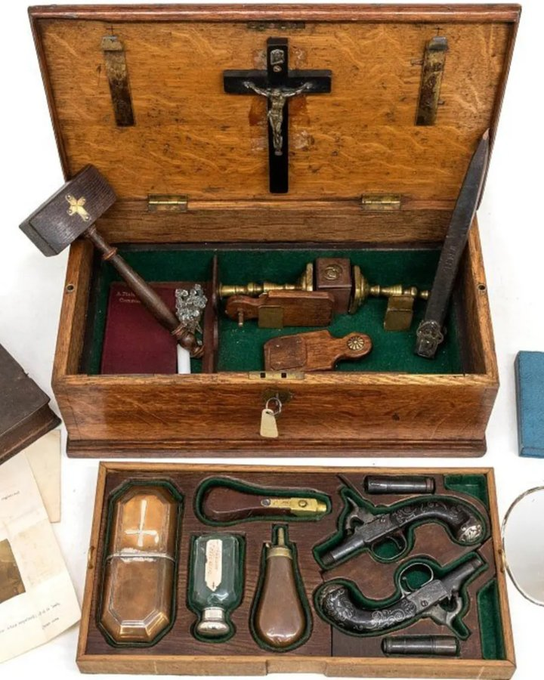
\includegraphics[width=0.5\linewidth]{imagens/VampireKillingSet.png}
    \caption{Caption}
    \label{fig:enter-label}
\end{figure}

\section{Itens Diversos de Apoio à Missão}

\begin{itemize}
    \item \textbf{Lanternas de Mão com Luz UV}: Para detecção de marcas, rastros ou inscrições ocultas que não são visíveis sob luz normal.

    \item \textbf{Rádio Comunicador de Longo Alcance}: Para manter a comunicação entre a equipe em locais isolados ou durante investigações noturnas.

    \item \textbf{Kit de Primeiros Socorros}: Inclui itens básicos para tratar ferimentos leves, desmaios e outros acidentes que possam ocorrer durante a missão.

    \item \textbf{Registro Digital e Anotação (Gravador de Voz e Canetas Marcadoras)}: Equipamentos para documentar observações e registros em campo.

    \item \textbf{Roupas de Proteção Contra o Frio e Máscaras de Proteção}: Equipamentos apropriados para ambientes úmidos ou com pouca ventilação, comuns em cavernas e túneis.
\end{itemize}

\section{Resumo dos Equipamentos para Missão}

A lista de equipamentos acima cobre as necessidades de uma investigação de assombrações, incluindo proteção espiritual, materiais de detecção e recursos tecnológicos para monitorar e coletar evidências. Com esses itens, a equipe terá recursos para garantir segurança e eficiência, maximizando as chances de sucesso na investigação dos fenômenos sobrenaturais.




